\reportheading{Appendix A.\quad Case register}
Propane results use FDS 6.10.1 and time-weighted means over 90--120~s. The four assigned base combinations comprise OP-1 and OP-6 at 47.2 and 106.2~kW. Reading the ordered HRRs in Peng et al., Table~2, gives Tests 4, 8, 44 and 48, respectively (low then high power within each door state). Successful FDS runs number 4, 9, 2 and 5 for these conditions, including grid, wall, model and diagnostic variants. The assignment table specifies eight cases but identifies only these four distinct even-group conditions. Propylene screening records extend to the first observed rejection or 120~s. The original-grid paired-flow comparison covers eight stations over 120~s; the refined 0.96~m$^3$/s OP-6 case stopped at its first recorded breach.
\subhead{Appendix B.\quad Grid and door-flow comparisons}
The characteristic fire diameters were 0.283 and 0.391~m at 47.2 and 106.2~kW. Their ratios to the longest cell dimensions were 5.65/7.82, 7.27/10.05 and 9.42/13.03 on the coarse, medium and fine meshes. Corresponding snapped burner areas were 0.06250, 0.06125 and 0.06300~m$^2$.
\tabletitle{B1. Doorway diagnostic cases, 90--120 s.}
\begin{reporttable}{L{.18}L{.20}L{.21}L{.21}L{.20}}
\rowcolor{tablegrey}Door&Fire (kW)&In (kg/s)&Out (kg/s)&RMSE (K)\\
OP-1&47.2&0.260&0.261&166.6\\
OP-1&106.2&0.318&0.322&55.0\\
OP-6&47.2&0.094&0.096&61.4\\
OP-6&106.2&0.095&0.098&361.4\\
\end{reporttable}
\reportfigure{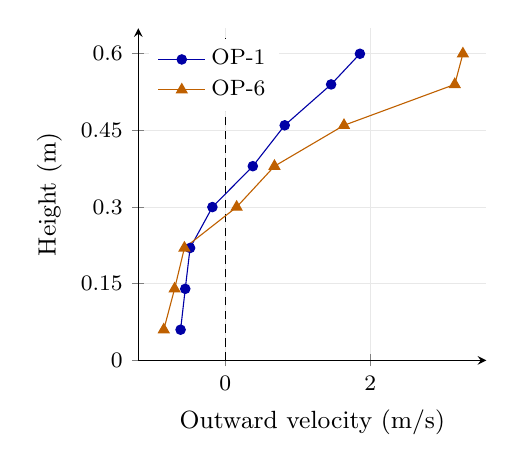
\begin{tikzpicture}
\begin{axis}[width=.495\linewidth,height=5.8cm,axis lines=left,ymin=0,ymax=.65,
ytick={0,.15,.30,.45,.60},xmin=-1.2,xmax=3.6,
xlabel={Outward velocity (m/s)},ylabel={Height (m)},grid=major,grid style={gray!18},
tick label style={font=\footnotesize},label style={font=\small},
legend style={at={(.03,.97)},anchor=north west,font=\footnotesize,draw=none}]
\addplot[black,densely dashed,forget plot] coordinates {(0,0) (0,.63)};
\addplot[blue!65!black,mark=*,mark size=1.7pt] coordinates {(-0.6169,0.06) (-0.5525,0.14) (-0.4858,0.22) (-0.1781,0.3) (0.3791,0.38) (0.8191,0.46) (1.459,0.54) (1.8563,0.6)};
\addlegendentry{OP-1}
\addplot[orange!75!black,mark=triangle*,mark size=2.2pt] coordinates {(-0.8488,0.06) (-0.6996,0.14) (-0.5641,0.22) (0.1562,0.3) (0.6777,0.38) (1.6367,0.46) (3.164,0.54) (3.2764,0.6)};
\addlegendentry{OP-6}
\end{axis}\end{tikzpicture}%
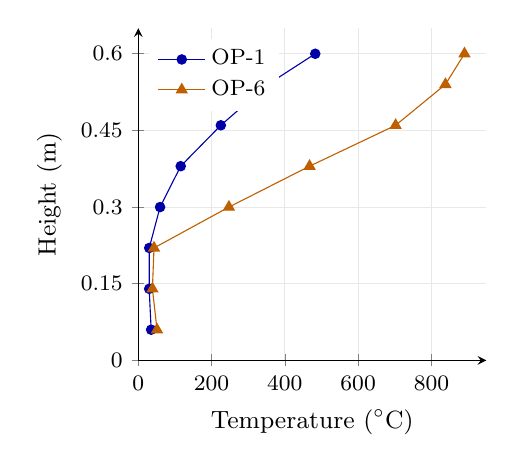
\begin{tikzpicture}
\begin{axis}[width=.495\linewidth,height=5.8cm,axis lines=left,ymin=0,ymax=.65,
ytick={0,.15,.30,.45,.60},xmin=0,xmax=950,
xlabel={Temperature ($^\circ$C)},ylabel={Height (m)},grid=major,grid style={gray!18},
tick label style={font=\footnotesize},label style={font=\small},
legend style={at={(.03,.97)},anchor=north west,font=\footnotesize,draw=none}]

\addplot[blue!65!black,mark=*,mark size=1.7pt] coordinates {(35.0545,0.06) (29.7306,0.14) (29.8055,0.22) (59.4344,0.3) (115.7244,0.38) (225.2291,0.46) (353.3391,0.54) (482.9451,0.6)};
\addlegendentry{OP-1}
\addplot[orange!75!black,mark=triangle*,mark size=2.2pt] coordinates {(51.0932,0.06) (38.5634,0.14) (42.8348,0.22) (247.3595,0.3) (467.4785,0.38) (702.2993,0.46) (838.2762,0.54) (890.311,0.6)};
\addlegendentry{OP-6}
\end{axis}\end{tikzpicture}}{Figure B1. R1 doorway profiles at eight elevations for the adiabatic 106.2~kW diagnostic runs. Each point is a 90--120~s average. Negative velocity denotes incoming air.}

\clearpage
\reportheading{Appendix C.\quad Original OP-6 search}
\tabletitle{C1. Sampled height margin (mm) as a function of curtain depth and flow.}
\begin{reporttable}{L{.28}L{.18}L{.18}L{.18}L{.18}}
\rowcolor{tablegrey}Curtain depth&\multicolumn{4}{c}{Total flow (m$^3$/s)}\\
(m)&0.08&0.16&0.24&0.32\\
0.00&$-334$&$-331$&$-295$&$-289$\\
0.08&$-336$&$-331$&$-288$&$-294$\\
0.16&$-335$&$-331$&$-296$&$-285$\\
0.24&$-336$&$-337$&$-294$&$-302$\\
\end{reporttable}
\clearpage
\reportheading{Appendix D.\quad Paired-flow data coverage}
\tabletitle{Table D1. Minimum thermal interface height (m) across eight stations, 0--120~s, original grid. The target is 0.380~m.}
\begin{reporttable}{L{.23}L{.23}L{.27}L{.27}}
\rowcolor{tablegrey}Door state&Soot (kg/kg)&0.96 m$^3$/s&1.28 m$^3$/s\\
OP-1&0.02&0.4574&\textbf{0.4425}\\
OP-1&0.05&0.4717&0.5093\\
OP-1&0.10&0.4410&0.5013\\
OP-6&0.02&\textbf{0.3957}&0.5827\\
OP-6&0.05&0.5262&0.4975\\
OP-6&0.10&0.4061&0.5503\\
\end{reporttable}
The 1.28~m$^3$/s minima in Table D1 were checked against the raw device histories and successful completion logs. At 0.96~m$^3$/s the archived per-station reductions cover eight stations and 0--120~s in each of the six cases. Some local raw folders contain earlier, interrupted runs. The low-flow comparisons use the archived full-duration station data.

\tabletitle{Table D2. Revised layout, OP-6, soot yield 0.02, 38-cell vertical grid. The minimum is taken over all eight stations in the recorded interval.}
\begin{reporttable}{L{.20}L{.22}L{.21}L{.37}}
\rowcolor{tablegrey}$Q$ (m$^3$/s)&Fan input (W)&Minimum (m)&FDS record\\
0.96&4.35&0.3717&Breach at 98.0 s\\
1.12&6.91&0.5522&Complete, 120 s\\
1.28&10.32&0.5429&Complete, 120 s\\
\end{reporttable}

Combined fan input uses the two short branches and efficiency of 0.60 in Section~2.2. The 1.12~m$^3$/s case minimises power in Table D2. Table D3 distinguishes cases that reached 120~s from those still accumulating device records. A recorded height below 0.38~m establishes a breach even before 120~s.
\tabletitle{Table D3. Refined-grid evidence at 1.12~m$^3$/s. Partial minima cover only the recorded interval.}
\begin{reporttable}{L{.16}L{.18}L{.21}L{.22}L{.23}}
\rowcolor{tablegrey}Door&Soot (kg/kg)&Status&Record (s)&Minimum (m)\\
\csname @@input\endcsname sections/intermediate-coverage.tex
\end{reporttable}
\clearpage
\reportheading{Appendix E.\quad Surrogate event scoring}
The physics-informed extreme learning machine used 96 fixed tanh units and a least-squares output fit with ridge coefficient 0.1. A simplified upper-layer volume balance constrained the weighted mean layer thickness under an assumption of lateral uniformity. A short event was a continuous excursion below 0.38~m at one station lasting at most 2~s. An event counted as a match when the intersection of the predicted and observed intervals covered at least half their union, with one-to-one matching. Linear interpolation between device records approximately 0.5~s apart limits the precision of short event durations.
\subhead{Testing the minimum-height decision directly}
On the earlier 20-case, 19-cell vertical grid cohort, whole-design holdout error in minimum height fell from 27.03 to 8.26~cm after fitting a station-minimum correction. Missed breaches fell from eight to six of eight, with one false alarm among twelve passing runs. Section~5 gives the expanded comparison.

For the refined OP-6 low-flow case, the corrected forecast frozen before completion was 0.4710~m. The 0.3717~m breach at 98~s gives an overprediction of at least 9.9~cm because the run stopped early. At 1.12~m$^3$/s, forecasts issued at 60 and 90~s identified the limiting station at $x=4.2$~m after its minimum at 49.50~s.

A separate two-second warning test used observations from running simulations. At a retrospectively matched count of 33 false alarms, local-height and multistation-temperature models detected the same four of 25 short events, with a mean lead of 0.73~s.

\reportfigure{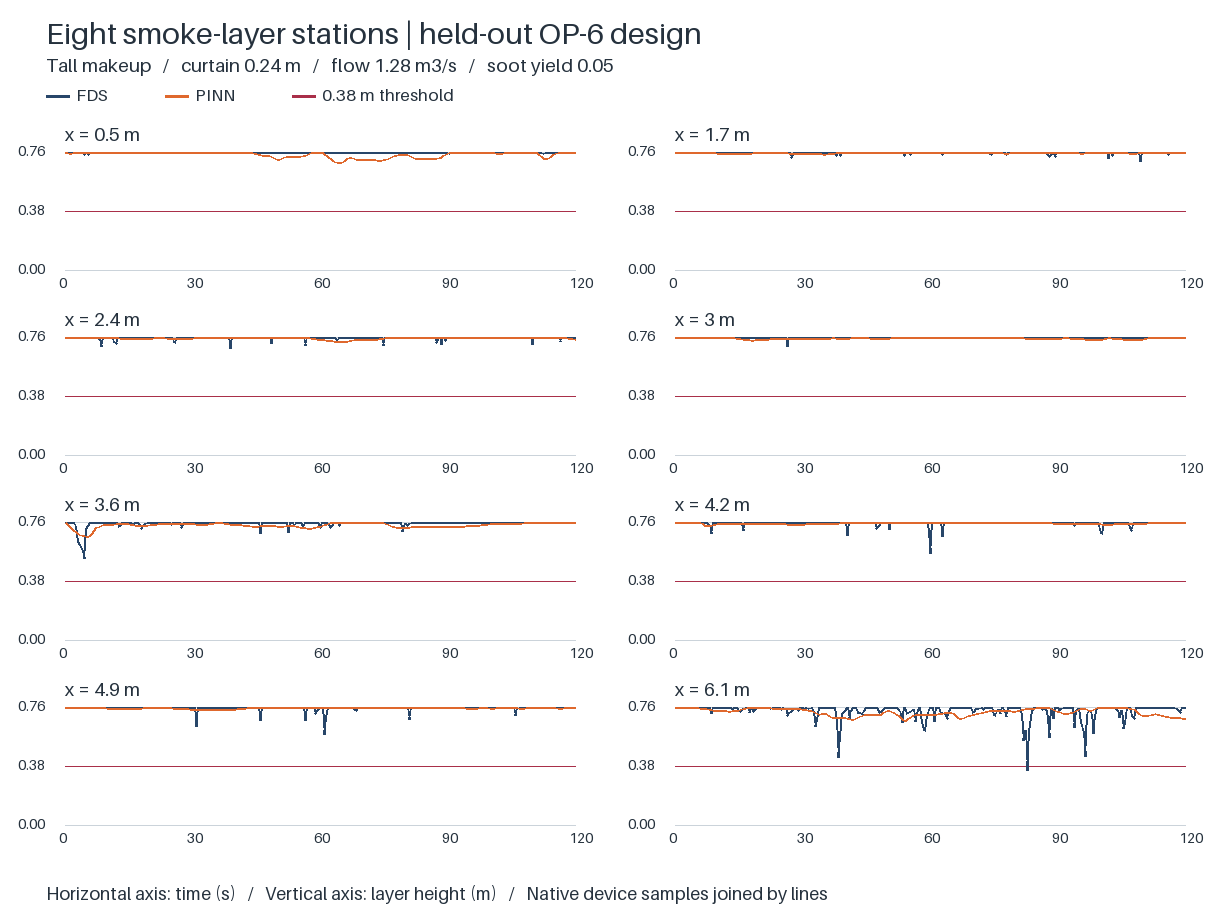
\includegraphics[width=.90\linewidth]{../../09_PINN_Layer/eight_stations.png}}{Figure E1. FDS and PINN thermal layer heights across the eight sampled columns. The far-end station is enlarged in Figure 5.}
